% These are the lecture notes for my CSCI360 course SPRING 2017
% at John Jay College of Criminal Justice. They are based largely on
% Schneier's Applied Cryptography.

% Feel free to edit these slides and use them for your own courses.
% HOWEVER DO NOT REMOVE THESE LINES!
% Email me at: awood [at] jjay.cuny.edu
% or at: awood [at] gradcenter.cuny.edu


\documentclass{beamer}

\usepackage{tikz}
\usetikzlibrary{calc}

\usepackage{forest}
\usepackage{verbatim}
\usepackage{color}
\usepackage{amsmath}
\usepackage{graphicx}
\usepackage{caption}



\setbeamertemplate{footline}[frame number]
\setbeamertemplate{navigation symbols}{} 

\newtheorem{thm}{Theorem}[section]
\newtheorem{lem}{Lemma}
\newtheorem{cl}{Claim}
\newtheorem{cor}{Corollary}[section]
\newtheorem{conj}{Conjecture}
\newtheorem{quest}{Question}
\newtheorem{defn}{Definition}[section]
\newtheorem{obs}{Observation}[section]
\newtheorem{exam}{Example}

\newcommand{\im}{\operatorname{im}}
\newcommand{\id}{\operatorname{id}}
\newcommand{\interior}{\operatorname{int}}
\newcommand{\bdry}{\operatorname{bdry}}
\newcommand{\<}{\langle}
\renewcommand{\>}{\rangle}
\newcommand{\Gab}{(G_\phi)^{ab}} 
\newcommand{\phibar}{\bar{\phi}}
\newcommand{\Z}{\mathbb{Z}}
\newcommand{\N}{\mathbb{N}}
\newcommand{\Q}{\mathbb{Q}}
\newcommand{\R}{\mathbb{R}}
\newcommand{\C}{\mathbb{C}}
\newcommand{\A}{\mathcal{A}}
\newcommand{\OO}{\mathcal{O}}
\newcommand{\UU}{\mathcal{U}}
\newcommand{\power}{2^{\{P_1, \cdots , P_n\}}}
\newcommand{\bp}{\begin{problem}}
\newcommand{\ep}{\end{problem}}
\newcommand{\ba}{\begin{answer}}
\newcommand{\ea}{\end{answer}}
\newcommand{\ds}{\displaystyle}
\newcommand{\ben}{\renewcommand{\theenumi}{\alph{enumi}}
\renewcommand{\labelenumi}{(\theenumi)}\begin{enumerate}}
\newcommand{\een}{\end{enumerate}}
\newcommand{\Hess}{\operatorname{Hessian}}
\newcommand{\Aut}{\mathrm{Aut}}
\newcommand{\Inn}{\mathrm{Inn}}
\newcommand{\Out}{\mathrm{Out}}
\newcommand{\End}{\mathrm{End}}


\mode<presentation>
{
%  \usetheme{default}
  \setbeamercovered{invisible}
}


\usepackage[english]{babel}
\usepackage[latin1]{inputenc}
\usepackage{times}
\usepackage[T1]{fontenc}
\usepackage{stmaryrd}

%\usetheme{default}
%\usetheme{AnnArbor}
%\usetheme{Antibes}
%\usetheme{Bergen}
%\usetheme{Berkeley}
%\usetheme{Berlin}
%\usetheme{Boadilla}
%\usetheme{CambridgeUS}
%\usetheme{Copenhagen}
%\usetheme{Darmstadt}
%\usetheme{Dresden}
%\usetheme{Frankfurt}
%\usetheme{Goettingen}
%\usetheme{Hannover}
%\usetheme{Ilmenau}
%\usetheme{JuanLesPins}
%\usetheme{Luebeck}
%\usetheme{Madrid}
%\usetheme{Malmoe}
%\usetheme{Marburg}
%\usetheme{Montpellier}
%\usetheme{PaloAlto}
%\usetheme{Pittsburgh}
%\usetheme{Rochester}
\usetheme{Singapore}
%\usetheme{Szeged}
%\usetheme{Warsaw}

%\usecolortheme{default}
%\usecolortheme{albatross}
\usecolortheme{beaver}
%\usecolortheme{beetle}
%\usecolortheme{crane}
%\usecolortheme{dolphin}
%\usecolortheme{dove} % grey, white, yellow
%\usecolortheme{fly} %grey, yellow
%\usecolortheme{lily} %white, yellow, blue
%\usecolortheme{orchid}
%\usecolortheme{rose}
%\usecolortheme{seagull}
%\usecolortheme{seahorse}
%\usecolortheme{whale}
%\usecolortheme{wolverine}

% Title page

\title[HF]{Message Authentication Codes (MACs)}

\subtitle{Based on \emph{Cryptography Engineering} by Schneier, Ferguson, Kohno, Chapter 6}

\author
{Lecture notes of Alexander Wood \\ \scriptsize \href{mailto:awood@jjay.cuny.edu}{awood@jjay.cuny.edu}}
\institute[JJay]{John Jay College of Criminal Justice}  

\date{}

\begin{document}

% Remove 'figure' text from figure captions 
\setbeamertemplate{caption}{\raggedright\insertcaption\par}

\begin{frame}
  \titlepage
\end{frame}


\begin{frame}
\frametitle{MACs}

A \textbf{message authentication code (MAC)} is a key-dependent one-way hash function.
\newline

They satisfy the same properties as one-way hash functions.\newline

In addition they have a \textbf{key}.
\end{frame}


\begin{frame}
\frametitle{MACs for Authentication}

MACs are used to \textbf{authenticate} files between users. It checks its \textbf{authenticity} (confirms the sender) as well as its \textbf{integrity} (it has not been tampered with). \newline

Sometimes a MAC is referred to as a Message Integrity Code (MIC), espcially in applications where MAC already stands for Media Access Control. 
\end{frame}


\begin{frame}
\frametitle{MAC Visualization}

\begin{figure}
\centering
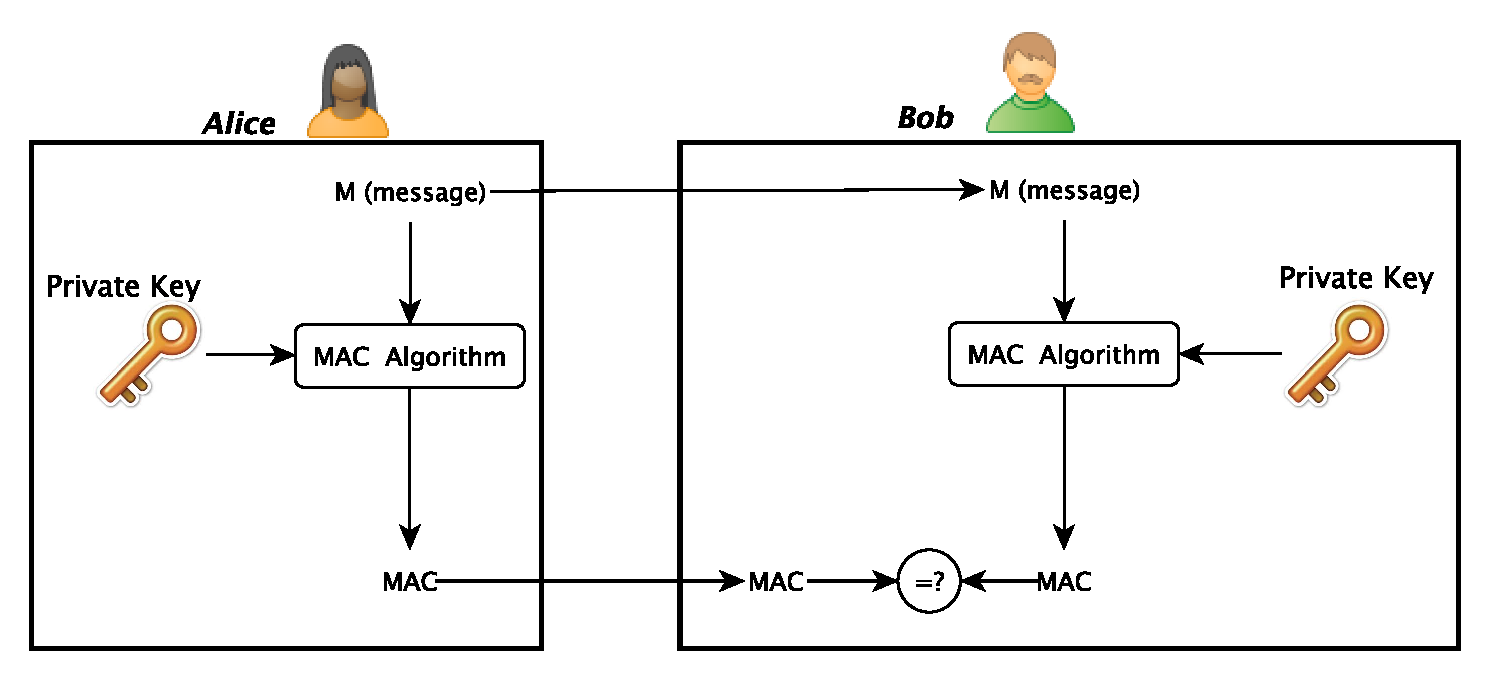
\includegraphics[scale=.45]{IMG/MAC}
\end{figure}
\end{frame}

\begin{frame}[fragile]
\frametitle{MAC Algorithms}

\begin{itemize}
\item \verb|KeyGen| - generates a key $1^n$ uniformly at random.
\item \verb|Sign| - Alice inputs her key $k$ and message $M$, receives output $t$ (tag).
\item \verb|Verify| - Bob verifies the authenticity of Alice's message.
\end{itemize}
\end{frame}


\begin{frame}
\frametitle{MACs}

A one-way hash function can be turned into a MAC by encrypting the hash function with a symmetric algorithm. \newline

Conversely, a MAC algorithm can be turned into a one-way hash function by changing the private key to a public key. 
\end{frame}


\begin{frame}
\frametitle{MAC Algorithms Visualization}

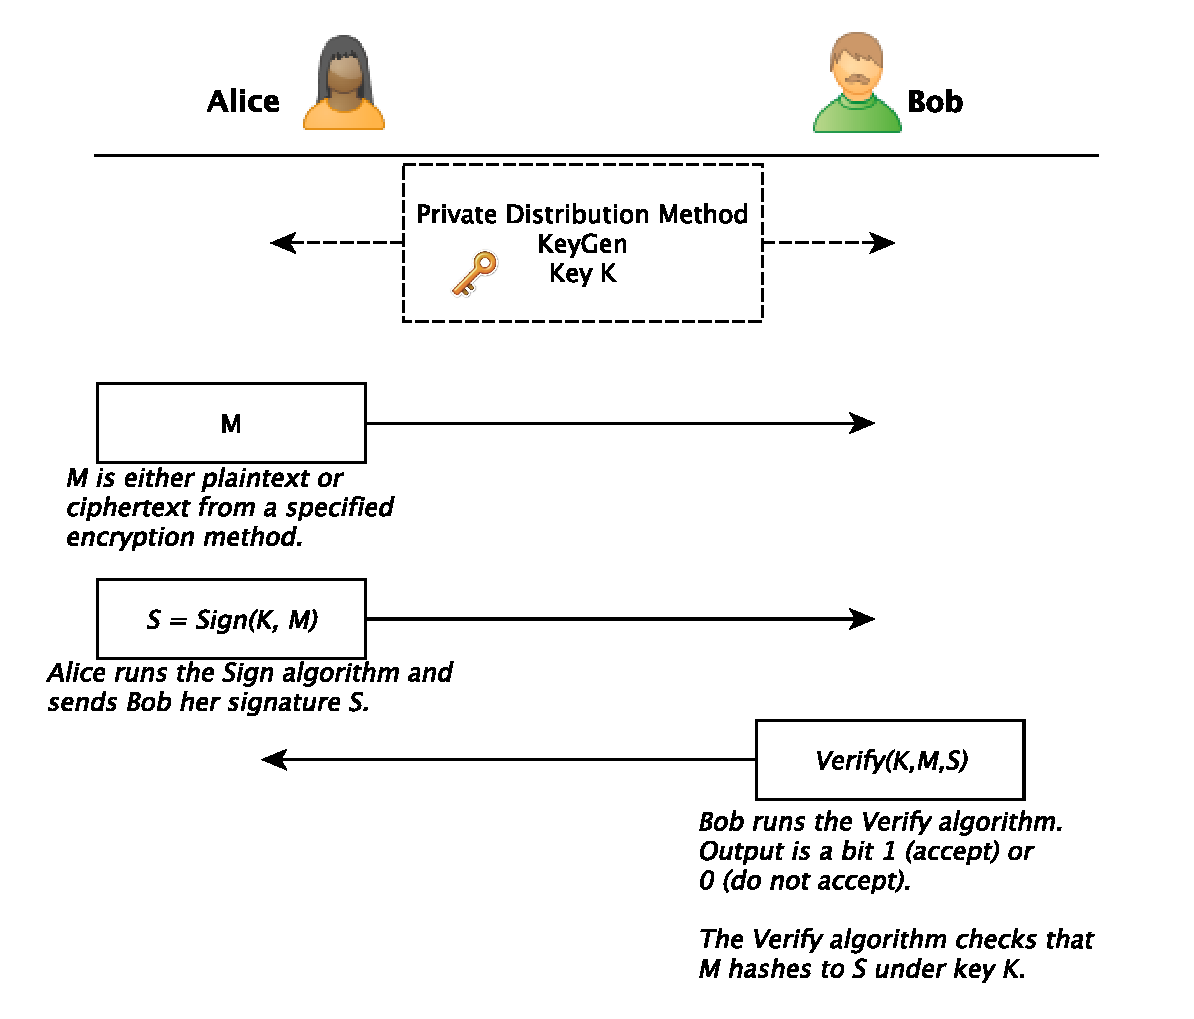
\includegraphics[scale=.45]{IMG/MACalg}
\end{frame}



\begin{frame}
\frametitle{MAC Security}

Again we take our security definition by \emph{Cryptography Engineering} by Ferguson, Schneier, and Kohno (Chapter 6).\newline

\begin{defn}
An \textbf{ideal MAC function} is a random mapping from all possible inputs (key, message pairs) to all possible $n$-bit outputs. 
\end{defn}

The attacker should \emph{not} know the entirety of the key. 
\end{frame}




\begin{frame}
\frametitle{Attack on a MAC}

While other security definitions exist, we will use the following broad one in this course. \newline

\begin{defn}
An \textbf{attack on a MAC} is a non-generic method of distinguishing the MAC from an ideal MAC function.\newline
\end{defn}

Recall that this is called a \textbf{distinguishing attack}. The idea is that the attacker should not be able to distinguish a valid signature from a random bitstring. Where have we seen this sort of attack before?
\end{frame}


\begin{frame}
\frametitle{Distinguishing Attack Visualization}

\begin{figure}
\centering
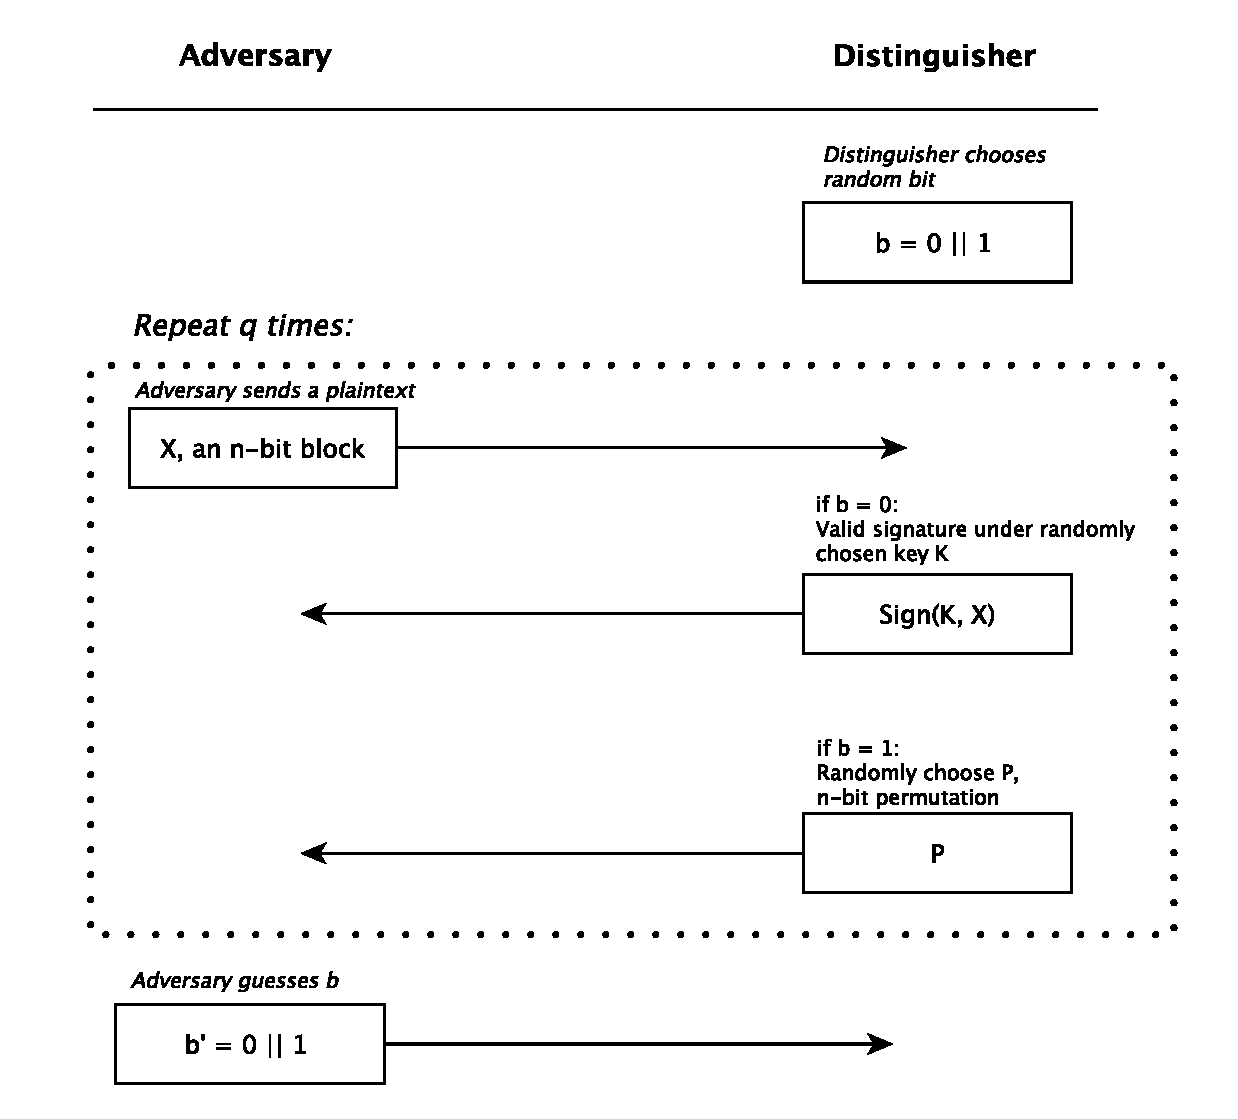
\includegraphics[scale=.4]{IMG/MACdistinguisher}
\end{figure}
\end{frame}



\begin{frame}
\frametitle{CBC-MAC}

\textbf{CBC-MAC} (cipher block chaining message authentication code) is a method of turning a block cipher into a MAC under a key $K$. The message is encrypted using cipher block chaining mode in order to create a construction where each block depends on the previous block.\newline

It is constucted as follows, where $M$ is split into length $n$ blocks $M_1, \dots, M_\ell$ and $E_k$ is  encryption under a key $K$.
\begin{align*}
H_0 &:= 0^n\\
H_i &:= E_K(M_i \oplus H_{i-1}) \\
MAC &:= H_\ell
\end{align*}
\end{frame}


\begin{frame}
\frametitle{CBC-MAC}

We saw something similar to this when constructing hash functions. Each hash block $H_i$ depends on the previous hash block $H_{i-1}$, constructed with a different block in the message.
\begin{figure}
\centering
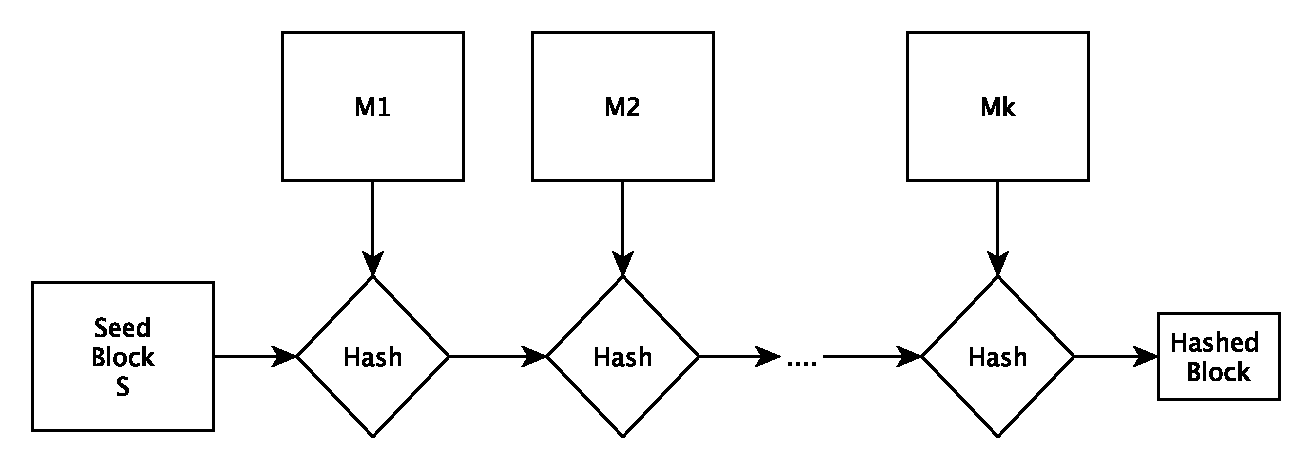
\includegraphics[scale=.5]{IMG/hash3}
\end{figure}
\end{frame}


\begin{frame}
\frametitle{CBC-MAC}

The difference now in \textbf{CBC-mode} is that we also must include a \textbf{key}. This requires a slightly different, though similar, construction.

\begin{figure}
\centering
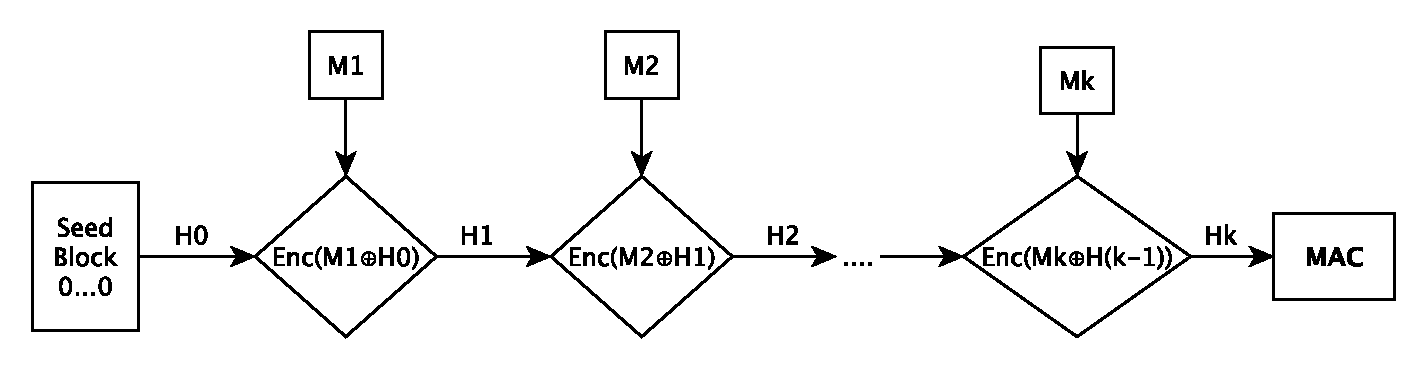
\includegraphics[scale=.45]{IMG/CBCMACchain}
\end{figure}
\end{frame}


\begin{frame}
\frametitle{Note On Keys}

Do NOT use the same key for encryption and authentication!

\begin{figure}
\includegraphics[scale=.4]{IMG/anotherone}
\end{figure}
\end{frame}


\begin{frame}
\frametitle{CBC-MAC}

CBC-MAC is secure for fixed-length messages \emph{if the underlying block cipher used is secure}.
\end{frame}


\begin{frame}
\frametitle{CBC-MAC: Collision Attack}

Let $M$ be a CBC-MAC function. Assume $M(a) = M(b)$. Then, $M(a\| c) = M(b\| c)$ where
\begin{align*}
M(a\| c) &= E_k(c\oplus M(a))\\
M(b\| c) &= E_k(c\oplus M(b))
\end{align*}

There are two stages to the attack.
\end{frame}

\begin{frame}[fragile]
\frametitle{CBC-MAC: Collision Attack, Step 1}

An attacker, Eve, collects MAC values until she finds a collision, ie, messages $a$ and $b$ such that $M(a) = M(b)$.\newline

According to the Birthday paradox, if we are using a \verb|128|-bit block cipher, this will take $2^{64}$ steps. 
\end{frame}


\begin{frame}
\frametitle{CBC-MAC: Collision Attack, Step 2}

Eve gets the sender, Alice, to authenticate the message $a\| c$. She can now replace this message with $b\|c$ without changing the MAC value. \newline

This means that the receiver, Bob, will accept the forged message $b\| c$.
\end{frame}


\begin{frame}
\frametitle{CBC-MAC: Collision Attack}

\begin{figure}
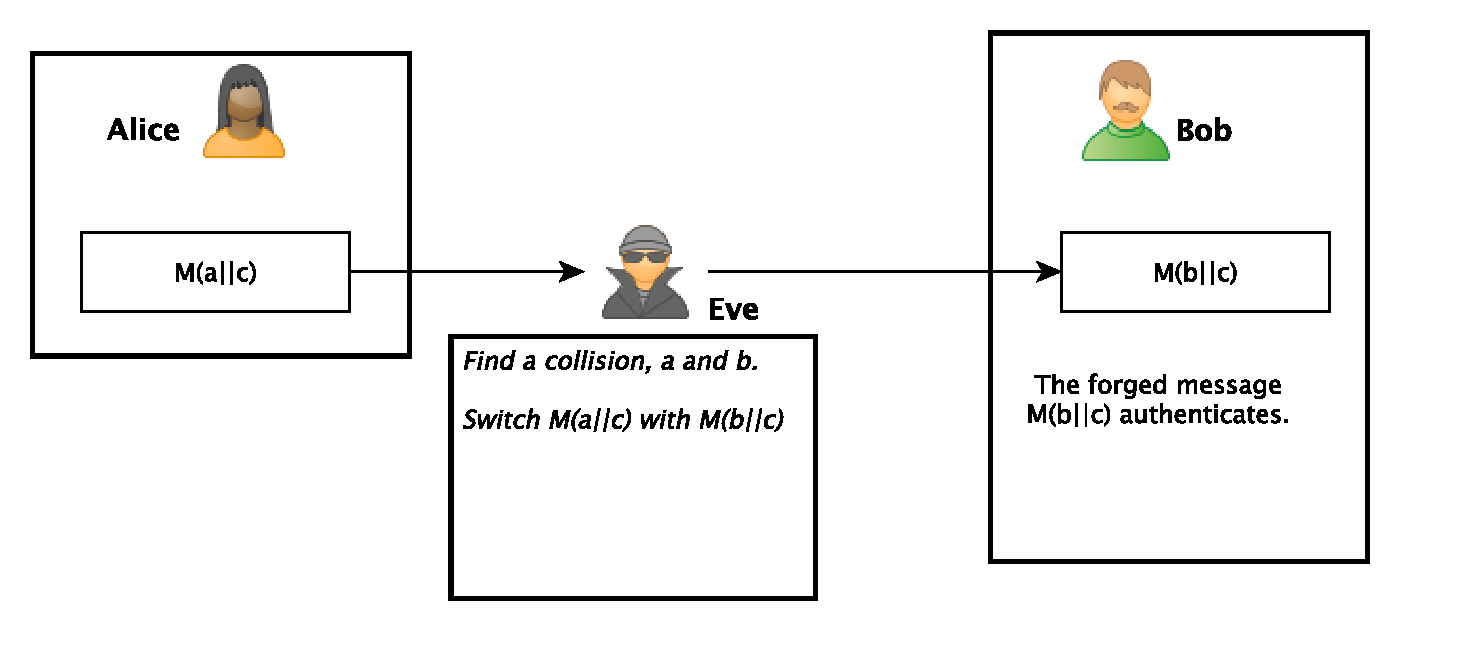
\includegraphics[scale=.45]{IMG/collisionattack}
\end{figure}
\end{frame}


\begin{frame}
\frametitle{CBC-MAC: Implementation}

If you wish to use CBC-MAC, follow the following steps.
\begin{enumerate}[1.]
\item Concatenate $\ell$ and $m$ to construct a string $s$, where $m$ is the message and $\ell$ is the length of $m$ encoded in a fixed-length format.
\item Pad $s$ until it is a multiple of the needed block size.
\item Apply CBC-MAC to the padded $s$.
\item Output the last ciphertext block. Do not output any intermediate values.
\end{enumerate}
\end{frame}



\begin{frame}
\frametitle{CMAC}

CMAC, also known as One-Key MAC and OMAC, is based off of CBC-MAC and was standardized by NIST in 2005.\newline

It fixes security deficiencies of CBC-MAC and is easier to implement with existing libraries in Python and Ruby.
\end{frame}

\begin{frame}[fragile]
\frametitle{CMAC}

CMAC works like CBC-MAC except on the last block. \newline

It derives two special values from its key and chooses one based on whether the length of the message is a multiple of the block length or not.\newline

It \verb|XOR|s one of two special values into the last block prior to the last block cipher encryption. 
\end{frame}



\begin{frame}
\frametitle{HMAC}

\textbf{HMAC} (keyed-hash message authentication code) uses a hash function to construct a MAC.\newline

HMACs are less affected by collision attacks than the hash functions which they are based off of. Hence, while MD5 is not colliion-resistant, HMAC-MD5 is considered to be reasonably safe as a MAC (as of 2011).
\end{frame}



\begin{frame}
\frametitle{HMAC}

HMAC computes:
\[
h((K\oplus a) \| h((K\oplus b)\|m))
\]
for constants $a$ and $b$, message $m$, key $K$, and hash function $h$. Note that $\|$ denotes concatenation.
\end{frame}

\begin{frame}
\frametitle{HMAC}

Note that:
\begin{itemize}
\item The message $m$ is only hashed once
\item The output is then hashed again with the key $K$
\item This HMAC construction works with any of the hash functions we discussed!
\end{itemize}
\end{frame}


\begin{frame}
\frametitle{Using A MAC}

Be careful when using a MAC! It is difficult to do properly.
\end{frame}


\begin{frame}[fragile]
\frametitle{Using a MAC}

Say Bob received \verb|Sign|$_K(m)$. Bob now knows that \emph{someone with the key $K$ approved the message $m$}. He knows nothing more than this.\newline

For example: Eve recorded a message signed by Alice and sent to Bob, then sent that same message to Bob at a later time. Bob then verified this message as being from Alice.
\end{frame}


\begin{frame}[fragile]
\frametitle{Using a MAC}

Suppose Alice and Bob want to authenticate a message $m$ along with data $d$ containing information such as the message number used, the source and destination of the message, etc. \newline

Frequently $d$ will be used as a header and concatenated to $m$. Then, $d\| m$ is signed and verified.
\end{frame}


\begin{frame}[fragile]
\frametitle{Using a MAC: The Horton Principle}

\textbf{The Horton Principle:} Authenticate what is \emph{meant}, not what is \emph{said}. 
\end{frame}

\begin{frame}
\frametitle{Using a MAC: The Horton Principle}

What is said is the bytes sent, and what is meant is the interpretation of the message. \newline

Thus the MAC should authenticate both the message $m$ as well as instructions on how to parse the message $m$. This can include a protocol identifier, version number, sizes for fields, et cetera.
\end{frame}


\begin{frame}
\frametitle{References}

\begin{itemize}
\item \emph{Applied Cryptography} By Schneier, Chapter 18
\item \emph{Cryptography Engineering} by Schneier, Ferguson, Kohno, Chapter 6
\end{itemize}
\end{frame}
\end{document}


